\newpage
\section{Вычеты, их вычисление. Вычисление контурных интегралов с помощью вычетов.}

\textbf{Вычетом} функции $f$ в точке $z_0$ называют число:
$$res\, f(z_0) = \frac{1}{2\pi i} \oint\limits_{\partial r}f(z)dz$$

\textbf{Вычисление вычетов:}
\textbf{Теорема о связи вычета с рядом Лорана:}

Пусть $f$ --- голоморфна в выколотой окрестности точки $a$. Тогда:
$$
res\, f(a) = c_{-1},
$$
где $f(z) = \sum_{n=-\infty}^{+\infty}c_n (z-z_0)^n$
\\

\begin{proof}
    \ \\
    $f(z)=\sum_{n=-\infty}^{+\infty}c_n(z-a)^n$ в $\overset{\circ}{U}_{\delta}(a)$, где $f\in H(\overset{\circ}{U}_{\delta}(a))$\\
    $\gamma_r=\{z: |z-a|=r\}, r\in (0, \delta)$, т.е. $\gamma_r \subset \overset{\circ}{U}_{\delta}(a)$\\
    Значит ряд сходится равномерно на $\gamma_r \Rightarrow $\\
    $\Rightarrow res\,f(z)=\frac{1}{2\pi i}\oint\limits_{\gamma_r}f(z)dz=\frac{1}{2\pi i}\sum_{-\infty}^{+\infty}\oint\limits{\gamma_r} c_n(z-a)^ndz=\frac{1}{2\pi i}c_{-1}\cdot 2\pi i$.
\end{proof}


\textbf{Следствие:}

В устранимой особой точке $z_0$: $res\, f(z_0) = 0$
\\

\textbf{Формула вычисления вычета в полюсе}

Пусть $z_0$ --- полюс функции $f$. Тогда:
$$
res\, f(z) = \frac{1}{(n-1)!} \underset{z \rightarrow z_0}{\lim} \left(f(z)(z-z_0)^n\right)^{(n-1)}
$$

\begin{proof}
    \ \\
    Разложение $f$ в ряд Лорана:\\
    $f(z)=\frac{c_{-n}}{(z-a)^n}+...+\frac{z_{-1}}{z-a}+c_0+c_1(z-a)+...$\\
    $f(z)\cdot (z-a)^n=c_{-n}+c_{-(n-1)}(z-a)+...+c_{-1}(z-a)^{n-1}+c_0(z-a)^n+...$\\
    $\left[f(z)\cdot (z-a)^n\right]^{(n-1)}=c_{-1}\cdot (n-1)!+\frac{n!}{1!}\cdot c_0\cdot (z-a)+...$\\
    При  $z\to a: $\\
    $\left[f(z)\cdot (z-a)^n\right]^{(n-1)}\rightarrow c_{-1}\cdot (n-1)! = (n-1)!res\,f(a)$
\end{proof}

\textbf{Следствие:}\\
Если $f(z)=\frac{\varphi(z)}{\psi(z)}$, где $\varphi, \psi$ -- голоморфны в точке $a$, $\psi(a)=0, \psi'(a)\neq 0$.\\
То $res\,f(a)=\frac{\varphi(a)}{\psi'(a)}$

\begin{proof}
    \ \\
    1.\\
    $\varphi(a)=0 \Rightarrow \lim\limits_{a\to a}f(z) = \lim\limits_{z\to a} \frac{\varphi'(z)}{\psi'(z)}=\frac{\varphi'(a)}{\psi'(a)} \in \mathbb{C} \Rightarrow a$ -- устранимая ос.т. $\Rightarrow res\,f(a)=0=\frac{\varphi(a)}{\psi'(a)}$\\
    2.\\
    $\varphi(a)\neq 0\Rightarrow \frac{1}{f(z)}=\frac{\psi(z)}{\varphi(z)}$ имеет в точке $a$ нуль первого порядка. Значит $a$ --- полюс 1-ого порядка. Тогда:\\
    $res\,f(a)=\lim\limits_{z\to a}\frac{\varphi(z)}{\psi(z)}(z-a)=\frac{\lim\limits_{z\to a}\varphi(z)}{\lim\limits_{z\to a}\frac{\psi(z)}{z-a}}=\frac{\varphi(a)}{\psi'(a)}$.
\end{proof}




\textbf{Теорема Коши о вычетах (вычисление контурных интегралов):}

Пусть $f \in H(D \backslash \{a_1 ... a_n\})$, где $a_1 ... a_n$ --- изолированные особые точки $f$,
$G \cup \partial G \subset D$, $\partial D$ не содержит особых точек $f$. Тогда:
$$
\oint\limits_{\partial G}f(z)dz = 2\pi i \sum_{i = 1}^{n} res\, f(a_i)
$$
(обход положительный)
\\

\begin{proof}
    \ \\
    Следует из теоремы Коши для многосвязной области:\\
    \begin{figure}[h]
        \centering
        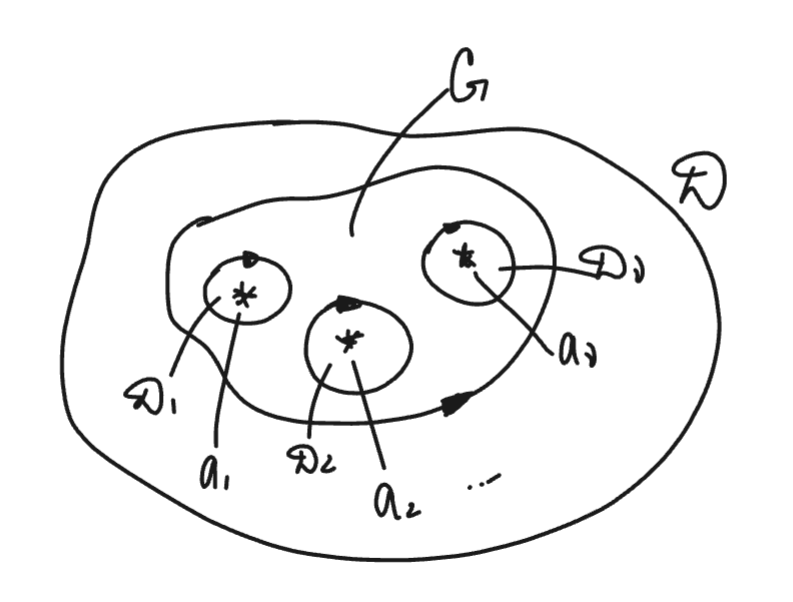
\includegraphics[width=1\linewidth]{answers/img/ans15.png}
    \end{figure}
    Окружности, окружающие $a_1, ..., a_\nu$ не пересекаются и лежат внутри $\partial G$.\\
    $\tilde{G}=G\backslash (D_1 \cup ...\cup D_\nu), f\in H(\tilde{G})$\\
    $\int\limits_{\partial \tilde{G}} f(z)dz = 0 \Rightarrow \int\limits_{\partial G}...+\sum_{j=1}^\nu \int\limits_{-\partial D_j}...=0 \Rightarrow$\\
    $\Rightarrow \int\limits_{\partial G}...-\sum_{j=1}^\nu 2\pi i \cdot res\, f(a_j)=0 \Rightarrow \int\limits_{\partial G}f(z)dz=2\pi i \sum_{j=1}^\nu res\,f(a_j)$.
\end{proof}
